%!TEX root = ./soutenance.tex


\section[Introduction]{Les codes polaires : construction et décodage}
\subsection*{Les codes correcteurs d'erreurs}

\begin{frame}[c]{Chaîne de communications numériques}
	\begin{center}
	\multiinclude[<+>][start=6,format=pdf,graphics={width=.8\textwidth}]{./fig/chaine_com}
	\end{center}
	\begin{itemize}
		\item<1-> Transmission de bits d'information
		\item<1-> Présence de perturbations
		\item<2-> Ajout de redondance
		\item<4-> Correction des erreurs
	\end{itemize}
\end{frame}

\begin{frame}
\vfill
	\begin{itemize}
		\item 1948 : Théorie de l’information (Shannon)
		\item 1950 : Codes de Hamming
		\item 1955 : Codes convolutifs
		\item 1960 : Codes BCH
		\item 1960 : Codes Reed-Solomon
		\item 1960 : \textbf{Codes LDPC (DVB,5G)}
		\item 1966 : Codes concaténés
		\item 1993 : \textbf{Turbocodes (4G)}
		\item 2008 : \textbf{Codes polaires (5G)}
	\end{itemize}
	\vfill
\end{frame}

\begin{frame}[c]
	\tableofcontents[
	subsectionstyle=hide,
	]
\end{frame}


\subsection*{Les codes polaires}
\begin{frame}[c]{Codes polaires}
	\begin{columns}[T] % align columns
		\begin{column}{.65\textwidth}
			\multiinclude[<+>][start=1,format=pdf,graphics={width=\textwidth}]{./fig/focus_polar}
		\end{column}
		\begin{column}{.35\textwidth}
		\begin{itemize}
			\item<1-> Matrice de codage
			\item<1->$F^{\otimes n}$ ; $F=\left[\begin{smallmatrix} 1 & 0 \\ 1 & 1\end{smallmatrix}\right]$
			\item<2-> Bits gelés
			\item<3-> Mot de code : $\mathbold{x}$
			\item<4-> Graphe de factorisation
		\end{itemize}
		\end{column}

	\end{columns}

\end{frame}
\subsection*{Le décodage SC}

\begin{frame}[c]{Décodage de codes polaires}
	\multiinclude[<+>][start=1,format=pdf,graphics={width=\textwidth}]{./fig/decoder_in_chain}    
	\begin{itemize}
		\item<2> Estimations, LLR (Log-Likelihood Ratio)
		\item<2> Signe, valeur binaire la plus probable
		\item<2> Valeur absolue, fiabilité de l'information
	\end{itemize}
\end{frame}

\begin{frame}[c]{Algorithme de décodage SC}
	\begin{columns}[T] % align columns
		\begin{column}{.55\textwidth}
			\multiinclude[<+>][start=1,format=pdf,graphics={width=\textwidth}]{./fig/focus_decoder}
		\end{column}
		\begin{column}{.45\textwidth}
		\begin{itemize}
			\item<1-> $L$ : Log Likelihood Ratios (LLR)
			\item<3-> $s$ : Sommes Partielles
		\end{itemize}
		\vspace{1cm}
			\only<4->{ \scriptsize{$$g(L_a,L_b,\hat{s}_a) = (1-2\hat{s}_a)L_a+L_b$$}}
			\only<5->{ \scriptsize{$$f(L_a,L_b) \approx \text{sign}(L_a.L_b).\min(|L_a|,|L_b|)$$}}
		\end{column}
	\end{columns}

\end{frame}

% \begin{frame}[c]{Algorithme de décodage SC}
% 	\begin{columns}[T] % align columns
% 		\begin{column}{.35\textwidth}
% 			\multiinclude[<+>][start=1,format=pdf,graphics={width=\textwidth}]{./fig/polar_functions}    
% 		\end{column}

% 		\begin{column}{.65\textwidth}
% 		\only<1>{
% 		$$f(L_a,L_b) \approx \text{sign}(L_a.L_b).\min(|L_a|,|L_b|)$$
% 		\vspace{1.1cm}

% 		$$g(L_a,L_b,\hat{s}_a) = (1-2\hat{s}_a)L_a+L_b$$
% 		}

% 				\only<2>{
% 				\vspace{0.5cm}
% 		$$\texttt{R1}(L_a)  =  \left\{\begin{array}{l c l} 0 \text{ si } L_a \geq 0 \\ 1 \text{ si } L_a < 0 \end{array}\right.$$
% 		\vspace{1.1cm}

% 		$$h(\hat{s}_a,\hat{s}_b) = (\hat{s}_{a} \oplus \hat{s}_{b}, \hat{s}_{b})$$
% 		}
% 		\end{column}

% 	\end{columns}

	
 %    g(L_a,L_b,\hat{s}_a)&=&(1-2\hat{s}_a)L_a+L_b\\
 %    h(\hat{s}_a,\hat{s}_b)&=& (\hat{s}_{a} \oplus \hat{s}_{b}, \hat{s}_{b})\\
 %    \texttt{R0}(L_a) &=& 0 \\
 %    \texttt{R1}(L_a) &=&  \left\{\begin{array}{l c l} 0 \text{ si } L_a \geq 0 \\ 1 \text{ si } L_a < 0 \end{array}\right.
% \end{frame}

% \begin{frame}[c]{Algorithme de décodage SC}
% 	\multiinclude[<+>][start=3,format=pdf,graphics={width=.8\textwidth}]{./fig/focus_decoder}
% \end{frame}

\begin{frame}[c]{Algorithme de décodage SC}
	\begin{columns}[T] % align columns

		\begin{column}{.55\textwidth}
			\multiinclude[<+>][start=2,format=pdf,graphics={width=\textwidth}]{./fig/sc_tree}

		\end{column}

		\begin{column}{.45\textwidth}
		\only<9>{
			\begin{itemize}
				\item \GREEN{Récursif et Régulier}
				\item \GREEN{Faible complexité}
				\item \GREEN{Bonnes performances pour de très grandes tailles de mots de code}
				\vspace{0.5cm}
				\item \RED{Performances modérées pour $N<4096$}
				\item \RED{Problème de propagation des erreurs}
			\end{itemize}
		}
		\end{column}

	\end{columns}

\end{frame}


\subsection*{Le décodage SC Liste}

\begin{frame}[c]{}
  	\frametitle<1-7>{Algorithme de décodage SCL}
  	\frametitle<8->{Algorithme de décodage CRC-SCL}

	\begin{columns}[T] % align columns
	\only<1-7>{
		\begin{column}{.7\textwidth}
	}
	\only<8->{
		\begin{column}{.6\textwidth}
	}
			\multiinclude[<+>][start=1,format=pdf,graphics={width=\textwidth}]{./fig/scl_anim}

		\end{column}
\only<1-7>
 {
		\begin{column}{.3\textwidth}
			\begin{itemize}
				\item<3-7> Pas de décision dure
				\item<4-7> Duplication des candidats
				\item<5-7> Métrique de candidats
				\item<6-7> Tri des métrique \& élimination
				\item<7-7> Mot de code décodé
			\end{itemize}
		\end{column}
}
\only<8->
 {
		\begin{column}{.4\textwidth}
			\begin{itemize}
				\item<8-> Concaténation d'un CRC
				\item<9-> Utilisé pour discriminer les candidats
			\end{itemize}
		\end{column}
}
	\end{columns}
\end{frame}


\begin{frame}[c]{Performances de décodage pour $N=2048,K=1723$}
	\centering
	\multiinclude[<+>][start=1,format=pdf,graphics={width=0.9\textwidth}]{./fig/scl_L/tikz/source}
\end{frame}

\begin{frame}[c]{Algorithmes adaptatifs}
	\centering
		\begin{columns}[T] % align columns
		\begin{column}{.55\textwidth}
			\multiinclude[<+>][start=1,format=pdf,graphics={width=\textwidth}]{./fig/adaptive}
		\end{column}
		\begin{column}{.45\textwidth}
		\begin{itemize}
			\vfill
			\item<3-> Partiellement adaptatif : PASCL (Partially Adaptive)
			\vfill
			\item<4-> Complètement adaptatif : FASCL (Fully Adaptive)
			\vfill
		\end{itemize}
		\end{column}

	\end{columns}

\end{frame}

\begin{frame}[c]{\'Elagage de l'arbre}
			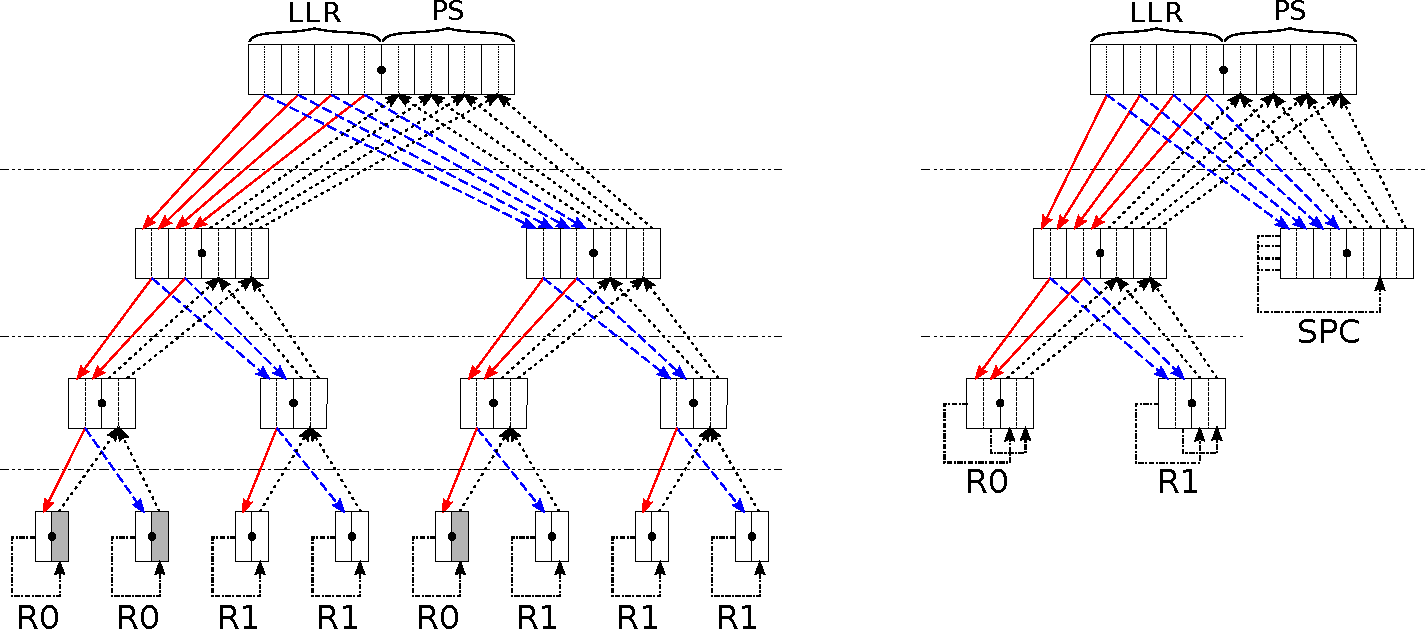
\includegraphics[width=\textwidth]{./fig/pruning}
\end{frame}
	
	\begin{frame}[c]{Résumé}
	\vspace{-0.5cm}
	\begin{minipage}[t][2cm][t]{\textwidth}
		\begin{itemize}
			\item<+-> Rôle des codes correcteurs d'erreurs
			\item<+-> Les codes polaires
			\item<+-> Compromis entre performances de décodage, débit et latence
		\end{itemize}
	\end{minipage}
	\vspace{0.5cm}	
	\begin{minipage}[t][2cm][t]{\textwidth}
	\only<3>{
		\begin{table}[t]
			\centering
			{\small\resizebox{0.8\linewidth}{!}{
			\begin{tabular}{r|c|c|c} 
				\textbf{Algorithme}  & \textbf{Performances}  & \multirow{2}{*}{\textbf{Débit}} & \textbf{Latence}  \\
				\textbf{de décodage} & \textbf{BER \& FER}    &                                 & \textbf{Maximum}  \\
				\hline
				SC           & \RED{faibles}                  & \GREEN{haut}                    & \GREEN{faible}    \\
				SCL          & \ORANGE{moyennes}              & \RED{bas}                       & \ORANGE{moyenne}  \\
				CRC-SCL       & \GREEN{élevées}            & \RED{bas}                       & \ORANGE{moyenne}  \\
				PASCL       & \GREEN{élevées}            & \GREEN{haut}                    & \ORANGE{moyenne}       \\
				FASCL       & \GREEN{élevées}            & \GREEN{haut}                    & \RED{forte}       \\
			\end{tabular}
			}}
		\end{table}
	}
	\end{minipage}

\end{frame}